\section{Software}
    \ \\
    \subsection{Aufbau}
    \ \\
    \begin{minipage}{\columnwidth}
      \makeatletter
      \def\@captype{figure}
      \makeatother
      \centering
      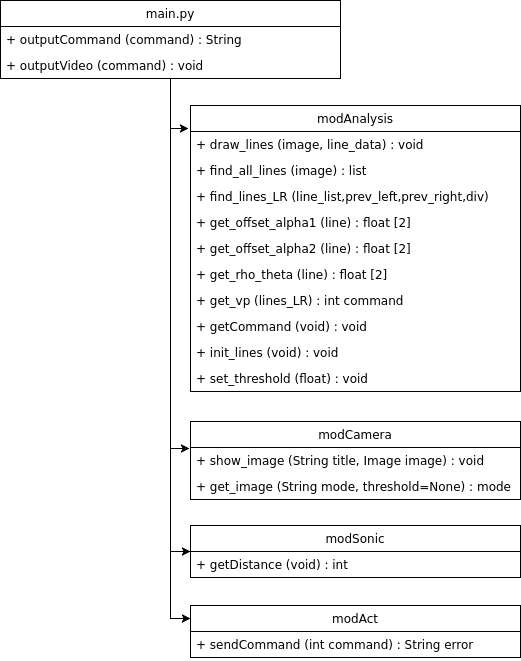
\includegraphics[width=0.8\linewidth]{images/code-flowchart.png}
      \caption{Aufbau des Python Codes}
      \label{fig:image-01}
    \end{minipage}
    \ \\

    \subsection{Externe Module}
    \ \\
    \begin{minipage}{\columnwidth}
      \makeatletter
      \def\@captype{table}
      \makeatother
      \centering
      %\rowcolors{1}{grey}{white}
      \begin{tabular}{ l | l }
      % \multicolumn{2}{|c}{Frame \#} & \multicolumn{4}{|c}{LCD 0/3} &
      Name & Beschreibung \\ \hline \hline
      tkinter & ... \\
      Adafruit\_PCA9685 & Bibliothek zur Ansteuerung des Motorcontrollers \\
      numpy & Bibliothek zur Verwendung von Matlab Funktionen \\
      cv2 & OpenCV 2 bietet Algorithmen zur Bildverarbeitung \\
      io & ... \\
      time & ... \\
      importlib & ... \\
      argparse & ... \\
      pivideostream & ... \\
      picamera & ... \\
      threading & ... \\
      RPi.GPIO & Bibliothek zur Ansteuerung der GPIO ports des Raspbery Pi \\
      \end{tabular}
      \caption{verwendete externe Python Module}
      \label{tab:01}
    \end{minipage}
    
    \subsection{Eigene Module}
    \ \\
    \begin{minipage}{\columnwidth}
      \makeatletter
      \def\@captype{table}
      \makeatother
      \centering
      %\rowcolors{1}{grey}{white}
      \begin{tabular}{ l | l }
      % \multicolumn{2}{|c}{Frame \#} & \multicolumn{4}{|c}{LCD 0/3} &
      Name & Beschreibung \\ \hline \hline
      modAnalysis & Verantwortlich für die eigentliche Verarbeitung der visuellen Informationen \\
      modAct & Verantwortlich für die Ansteuerung des Motors und der Lenkung \\
      modCamera & Bereitet das Kamerabild für die Verarbeitung und Anzeige vor. \\
      modSonic & Kommuniziert mit dem Ultraschallsensor und liefert Distanz zum Hindernis.\\
      \end{tabular}
      \caption{verwendete eigene Python Module}
      \label{tab:01}
    \end{minipage}

